\documentclass{article}
\usepackage{amsmath}
\usepackage{amssymb}
\usepackage{graphicx}
\usepackage{hyperref}
\usepackage[version=4]{mhchem}

\title{Example 1}
\date{}

\begin{document}
\maketitle

Triangle \(A B C\) is an isosceles triangle. \(D\) is a point the on \(A B\). Extend \(A C\) to \(E\) and connect \(D E\) so that \(B D=C E\). Prove: \(D F=F E\).

Proof:
Method 1:\\
Draw \(D G / / C E\). We have ,\\
\centering
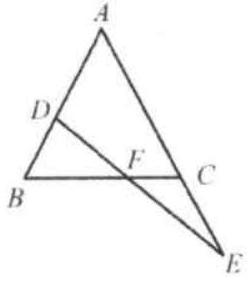
\includegraphics[width=\textwidth]{images/102.jpg}\\
\(\angle B=\angle D G B=\angle C\). So \(B D=D G=C E\).\\
We also know that \(\angle G D F=\angle C E F, \angle D G F=\angle E C F\).\\
Thus \(\triangle D G F \cong \triangle E C F(A S A)\).\\
So \(D F=F E\).\\
\centering
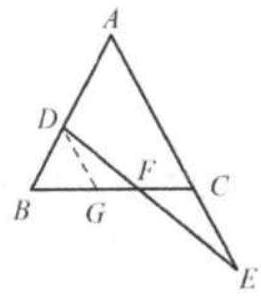
\includegraphics[width=\textwidth]{images/102(2).jpg}

Method 2:\\
Draw \(E G / / B G\) to meet the extension of \(B C\) at \(G\).\\
We see that \(\angle B=\angle G=\angle A C B=\angle E C G\), so \(C E=G E=B D\).\\
In \(\triangle D F B\) and \(\triangle E F G, \angle B D F=\angle G E F, G E=B D, \angle B=\angle G\).\\
Thus \(\triangle D F B \cong \triangle E F G(A S A)\).\\
\centering
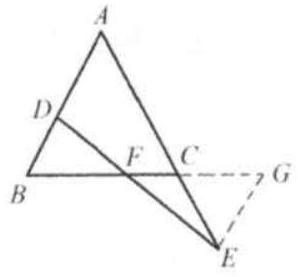
\includegraphics[width=\textwidth]{images/102(3).jpg}

So \(D F=F E\).

Method 3:\\
Draw \(D G / / B C\).\\
Since triangle \(A B C\) is an isosceles triangle, we know that \(B D=\) \(C G=C E\). Thus \(C, F\) are midpoints of \(E G, E D\), respectively.\\
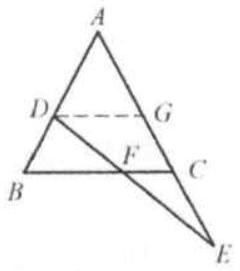
\includegraphics[width=\textwidth]{images/102(1).jpg} So \(C F\) bisects and \(D F=E F\).


\end{document}
